\section{Auswertung}
\label{sec:Auswertung}
\subsection{Bestimmung der spezifische Ladung der Elektronen}
In diesem Versuchteil werden die spezifische Ladung der Elektronen mittels  einer  großen  Helmholtz-Spule.\\
Die Windungszahl beträgt $\text{N}=20 \,\text{Windungen}$ und der Spulenradius ist $\text{R}=0,282 \, \text{m}$.\\
Der Weg der Elektronen, auf dem das Magnetfeld wirksam ist (Abstand zum Leuchtschirm), beträgt $\text{L}=17,5 \text{cm}$ \cite{AL}.\\
Das Spulenstrom I in Abhängigkeit von der Strahlverschiebung D wird jeweils für die Beschleunigungspannung von $\text{U}_\text{B}$ = 250 und 420 V  gemessen.\\
Die  Flussdichte  B  des  Helmholtz-Feldes wird durch Gleichung (6) berechnet.\\
Diese Messwerte und berechneten Werte sind in Tabelle \ref{tab:spe} aufgelistet.

 \begin{table}[H]
    \centering
    \caption{Die Mess und berechnete-Daten zur Bestimmung der spezifische Ladung der Elektronen.}
    \label{tab:spe}
    \begin{tabular}{| c | c |c|  c |c|c|}
    \toprule
    $\text{D}/10^{-3}\text{m}$& $\dfrac{\text{D}}{\text{L}^2+\text{D}^2}\Big/ \dfrac{1}{\text{m}}$&\multicolumn{2}{c|}{$\text{I}/\text{A}$}& \multicolumn{2}{c|}{$\text{B}/\mu \text{T}$}\\[2ex]
    \cline{3-6}
    &&&&& \\[\dimexpr-\normalbaselineskip+2pt]
    {}&{}&$\text{U}_\text{B}=250\text{V}$&$\text{U}_\text{B}=420\text{V}$&$\text{U}_\text{B}=250\text{V}$&$\text{U}_\text{B}=420\text{V}$\\
    \midrule
 0  	&0    	&0  	&0    &  0    	&  0    \\
 6,35	&0,207	&0,25	&0,20	& 15,943	& 12,754\\
12,70	&0,413	&0,60	&0,62	& 38,263	& 39,538\\
19,05	&0,615	&0,95	&1,05	& 60,583	& 66,960\\
25,40	&0,812	&1,25	&1,50	& 79,714	& 95,657\\
31,75	&1,004	&1,58	&1,90	&100,759	&121,166\\
38,10	&1,188	&1,92	&2,35	&122,441	&149,863\\
44,45	&1,363	&2,28	&2,27	&145,399	&144,761\\
50,80	&1,530	&2,60	&3,25	&165,806	&207,257\\

    \bottomrule
 \end{tabular}
\end{table}
\noindent
Die Regressionen zur Bestimmung der spezifische Ladung der Elektronen werden in \autoref{fig:plot} veranschaulicht.
\begin{figure}[H]
  \centering
  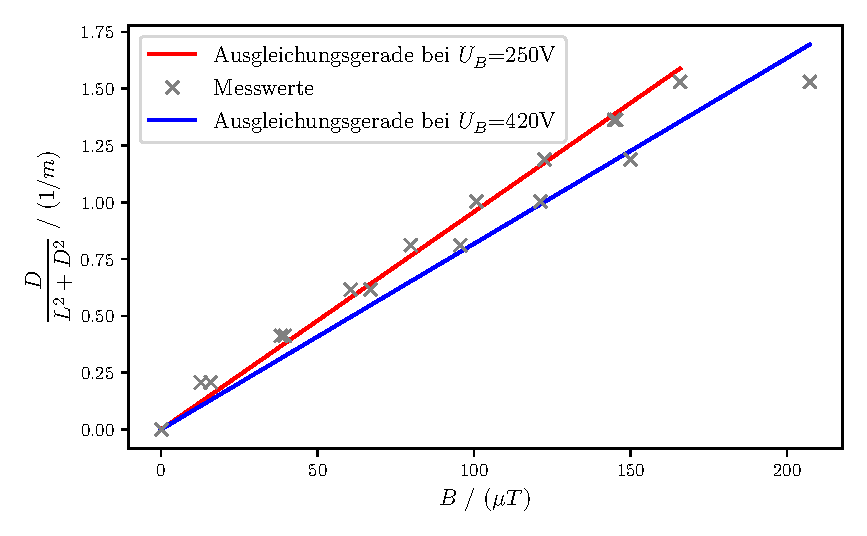
\includegraphics{plot.pdf}
  \caption{Die Regressionen zur Bestimmung der spezifische Ladung der Elektronen.}
  \label{fig:plot}
\end{figure}
\noindent
Die Ausgleichungsgeraden haben die Form:
\begin{equation}
 \text{y}=\dfrac{1}{\sqrt{8\text{U}_\text{B}}}\sqrt{\text{a}}\cdot \text{x}.\\
\end{equation}
mit \begin{align*}
   \text{y}=\frac{\text{D}}{\text{L}^2+\text{D}^2},\,\, \text{x}=\text{B}  \,\,\text{und}\, \,\text{a}=\frac{\text{e}_0}{\text{m}_0}.\\
  \end{align*}
 Die spezifische Ladung der Elektronen entspricht dem Parameter a und ergibt 
 \begin{align*}
  \text{für U}_\text{B}=250 \,\text{V} &:\frac{\text{e}_0}{\text{m}_0} =\text{a}=(1,83685 \pm 0,05613)\, 10^{11}\,\mathrm{\frac{C}{kg}}\\
  \text{für U}_\text{B}=420 \,\text{V} &:\frac{\text{e}_0}{\text{m}_0}=\text{a} =(2,24675 \pm 0,16591)\,10^{11}\,\mathrm{\frac{C}{kg}}.\\
 \end{align*}



 \subsection{Bestimmung der Intensität des lokalen Erdmagnetfeldes}
 Bei der Beschleunigungspannung ($\text{U}_\text{B}$ =200 V) wird die Lage des Leuchfleckes im xy-Koordinaten beobachtet und notiert (Das Helmholtz-Feld ist aus).
Zuerst wird die Achse der Röhre in Nord-Süd-Richtung und in Ost-West-Richtung gedreht. 
Die Elektronen werden durch Wirchkung des Erdfeldes in y-Richtung gelenkt.\\
 Das Helmholtz-Feld wird  dann eingeschaltet und dessen Strom $\text{I}_{\text{hor}}$ wird solange verändert, bis ihr Magnetfeld das der Erde kompensiert hat.
Die Horizontalkomponente $\text{B}_{\text{hor}}$ des Erdfeldes ist daher gleich dem Helmholtz-Feld.
Aus dem Spulenstrom $\text{I}_{\text{hor}}=0,5\, \text{A}$ lässt sich die Horizontalkomponente $\text{B}_{\text{hor}}$ des Erdfeldes durch Gleichung (6) errechnen.
Somit ist $\text{B}_{\text{hor}}=3,189 \,\mu \text{T}$.\\
Die Totalintensität $\text{B}_{\text{total}}$ des lokalen Erdmagnetfeldes wird durch
\begin{equation}
  \text{B}_{\text{total}}=\text{B}_{\text{hor}}\cdot \text{cos}(\varphi)\\
 \end{equation}
mit dem Inklinationswinkel $\varphi$ bestimmt.
Bei dem Veruschteil konnte der Inklinationswinkel $\varphi$ nicht bestimmt werden. 




